% !TEX TS-program = xelatex
% !BIB program = bibtex
% !TeX spellcheck = ru_RU
% !TEX root = talk.tex

\documentclass
  [ russian
  , aspectratio=169 % Для защит онлайн лучше использовать разрешение не 4х3
  ] {beamer}

%%% Обязательные пакеты
%% Beamer
\usepackage{beamerthemesplit}
\usetheme{SPbGU}
\beamertemplatenavigationsymbolsempty
\usepackage{appendixnumberbeamer}

%% Локализация
\usepackage{fontspec}
\setmainfont{CMU Serif}
\setsansfont{CMU Sans Serif}
\setmonofont{CMU Typewriter Text}
%\setmonofont{Fira Code}[Contextuals=Alternate,Scale=0.9]
%\setmonofont{Inconsolata}
% \newfontfamily\cyrillicfont{CMU Serif}

\usepackage{polyglossia}
\setdefaultlanguage{russian}
\setotherlanguage{english}
\usepackage[autostyle]{csquotes} % Правильные кавычки в зависимости от языка

%% Графика
\usepackage{wrapfig} % Позволяет вставлять графику, обтекаемую текстом
\usepackage{pdfpages} % Позволяет вставлять многостраничные pdf документы в текст

%% Математика
\usepackage{amsmath, amsfonts, amssymb, amsthm, mathtools} % "Адекватная" работа с математикой в LaTeX

% Математические окружения с русским названием
\newtheorem{rutheorem}{Теорема}
\newtheorem{ruproof}{Доказательство}
\newtheorem{rudefinition}{Определение}
\newtheorem{rulemma}{Лемма}

%%% Дополнительные пакеты. Используются в презентации, но могут быть отключены при необходимости
\usepackage{tikz} % Мощный пакет для создание рисунков, однако может очень сильно замедлять компиляцию
\usetikzlibrary{decorations.pathreplacing,calc,shapes,positioning,tikzmark}

\usepackage{multirow} % Ячейка занимающая несколько строк в таблице

%% Пакеты для оформления алгоритмов на псевдокоде
\usepackage[noend]{algpseudocode}
\usepackage{algorithm}
\usepackage{algorithmicx}

\usepackage{fancyvrb}

\NewDocumentCommand{\xxHash}{}{\textsc{xxHash}}
\NewDocumentCommand{\riscv}{}{\textsc{RISC-V}}
\NewDocumentCommand{\xxh}{m}{\textsc{XXH{#1}}}
\NewDocumentCommand{\sew}{}{\textsc{SEW}}
\NewDocumentCommand{\vl}{}{\textsc{VL}}
\NewDocumentCommand{\rvv}{}{\textsc{RVV}}
\usepackage{booktabs}
\usepackage{tabularx}
\usepackage{siunitx} % для таблиц с единицами измерений

\setbeamertemplate{itemize items}[circle]
\setbeamertemplate{enumerate items}[circle]

\newcommand\blfootnote[1]{%
	\begingroup
	\renewcommand\thefootnote{}\footnote{#1}%
	\addtocounter{footnote}{-1}%
	\endgroup
}

\makeatletter

\input{pretitle.tex}
\input{title.tex}

\newcommand{\academicGroup}{\my@title@group@ru}
\newcommand{\advisorChair}{\my@title@chair@ru}
% То, что в квадратных скобках, отображается внизу по центру каждого слайда.
\title[Lamagraph: Транслятор в Interaction Nets]{\my@title@title@ru}
% То, что в квадратных скобках, отображается в левом нижнем углу.
\author[\my@title@author@ru]{\my@title@author@ru, группа \academicGroup}
\institute[СПбГУ]{}
\date[25 апреля 2025 г.]{}
\newcommand{\supervisor}{\my@title@supervisor@ru}
\newcommand{\supervisorPosition}{\my@title@supervisorPosition@ru}
\newcommand{\consultant}{\my@title@consultant@ru}
\newcommand{\consultantPosition}{\my@title@consultantPosition@ru}
\newcommand{\reviewer}{\my@title@reviewer@ru}
\newcommand{\reviewerPosition}{\my@title@reviewerPosition@ru}
\newcommand{\defenseYear}{\my@title@year@ru}

\makeatother
\begin{document}
{
\setbeamertemplate{footline}{}
% Лого университета или организации, отображается в шапке титульного листа
\begin{frame}
    \includegraphics[width=1.4cm]{figures/герб_серый.png}
    \vspace{-35pt}
    \hspace{-10pt}
    \begin{center}
        \begin{tabular}{c}
            \scriptsize{Санкт-Петербургский государственный университет} \\
            \scriptsize{\advisorChair}
        \end{tabular}
        \titlepage
    \end{center}

    \btVFill

    {\scriptsize
        % У научного руководителя должна быть указана научная степень
        \textbf{Научный руководитель:} \supervisorPosition~\supervisor \\
        % Консультанта может и не быть. Должна быть указана должность или ученая степень
        % \textbf{Консультант:}  \consultantPosition~\consultant \\
        % Для учебной практики не обязателен. Должна быть указана должность или ученая степень
        \textbf{Рецензент:} \reviewerPosition~\reviewer \\
    }
    \makeatother
    \begin{center}
        \vspace{5pt}
        \scriptsize{Санкт-Петербург\\ \defenseYear}
    \end{center}
\end{frame}
}

\begin{frame}{Введение}

    \begin{itemize}
        \item Задачи искусственного интеллекта и анализа графов влекут за собой нерегулярный параллелизм
        \item Традиционные архитектуры плохо справляются с нерегулярным параллелизмом $\implies$~требуются специализированные ускорители
        \item \INs{}~--- модель вычислений, которой естествен нерегулярный параллелизм
        \item Существуют программные реализации \INs{}, однако попыток реализовать ускоритель на её основе пока не предпринималось
    \end{itemize}

\end{frame}

\begin{frame}{\Lamagraph{}}

    Проект \Lamagraph{} исследует возможности по разработке
    \begin{itemize}
        \item параметризуемого многоядерного сопроцессора на основе \INs{}
        \item ML-подобного функционального языка для программирования сопроцессора
    \end{itemize}
    \begin{center}
        \includegraphics[width=\linewidth]{figures/lamagraph-big-horiz.pdf}
    \end{center}

\end{frame}

\begin{frame}{Состояние проекта}

    Проект на первом этапе: разработка минимальной инфраструктуры для создания ускорителей на основе Interaction Nets

    \vspace{1em}

    На данном этапе от проекта ожидается следующее
    \begin{itemize}
        \item Приоритизация получения полнофункционального прототипа, содержащего все компоненты
        \item Использование единого стека технологий: Clash $\implies$ Haskell
        \item Возможность анализа результатов каждого этапа работы
    \end{itemize}

\end{frame}

\begin{frame}
    \frametitle{Постановка задачи}

    \textbf{Целью} работы является разработка транслятора модельного функционального языка в \INs{}
    \vspace{1em}

    \textbf{Задачи}:
    \begin{enumerate}
        \item Реализовать интерпретатор модельного ML-подобного языка
              \begin{itemize}
                  \item Фронтенд транслятора
                  \item Интерпретатор обогащенного $\lambda$-исчисления
              \end{itemize}
        \item Реализовать транслятор $\lambda$-исчисления в \INs{}
        \item Реализовать интерпретатор \INs{}, поддерживающий сбор метрик исполнения
    \end{enumerate}

\end{frame}

\begin{frame}
    \frametitle{Реализация}

    \begin{center}
        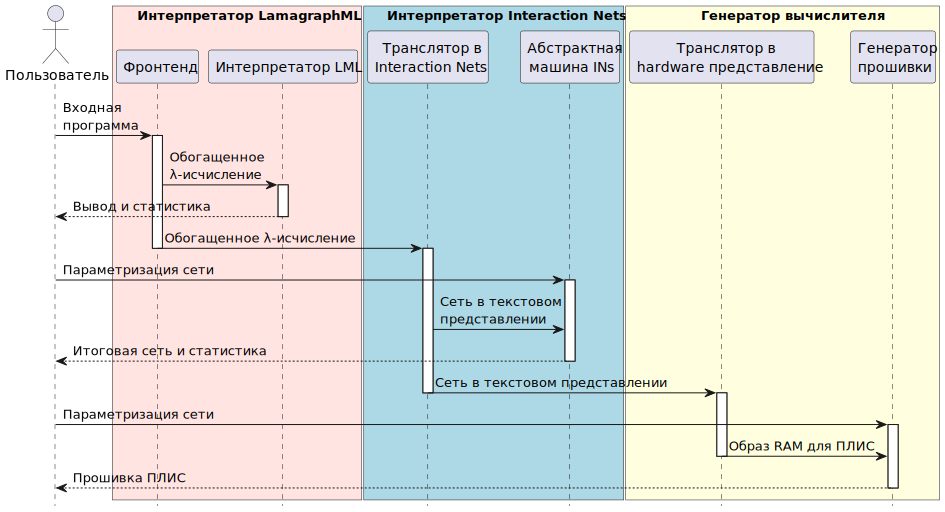
\includegraphics[width=0.8\linewidth]{figures/using.pdf}
    \end{center}

\end{frame}

\begin{frame}{Фронтенд и интерпретатор LamagraphML}

    \begin{itemize}
        \item Используется ML-подобный синтаксис, для представления AST используется паттерн Trees That Grow
        \item Парсер реализован с помощью связки \textsc{Alex} и \textsc{Happy} с применением property-based тестов
        \item Используется система типов Хиндли-Милнера
        \item Для упрощения дальнейших преобразований используется промежуточное представление~--- обогащенное $\lambda$-исчисление
        \item Реализован интерпретатор на основе замыканий, на данный момент он наследует стратегию языка реализации~--- call-by-need
    \end{itemize}

\end{frame}

\begin{frame}
    \frametitle{Транслятор $\lambda$-исчисления в \INs{}}

    \begin{itemize}
        \item Существует не одна схема трансляции $\lambda$-исчисления в \INs{}
        \item Используем схему, реализующую стратегию вычислений call-by-value
        \item Выяснилось, что схемы трансляции разрабатываются только для чистого $\lambda$-исчисления
              \begin{itemize}
                  \item Существующие расширения не подходят в нашем случае
                  \item Реализована поддержка только чистого $\lambda$-исчисления
              \end{itemize}
        \item Расширения схемы трансляции~--- предмет дальнейшей работы
    \end{itemize}

\end{frame}

\begin{frame}
    \frametitle{Интерпретатор \INs{}}

    \begin{columns}
        \begin{column}{0.6\linewidth}
            \begin{itemize}
                \item Стандартное представление \INs{}~--- графовое
                \item Работать с графами в функциональных языках сложно $\implies$ используем альтернативное текстовое представление
                \item Для него существует абстрактная машина, она и была реализована
            \end{itemize}
        \end{column}
        \begin{column}{0.35\linewidth}
            Графовое представление:

            \begin{center}
                \includegraphics[width=0.5\linewidth]{figures/ins_graph.pdf}
            \end{center}

            Текстовое представление
            \[\big\langle x \mid{} \Downarrow(x) \bowtie \lambda(y, y) \big\rangle\]
        \end{column}
    \end{columns}

\end{frame}

\begin{frame}
    \frametitle{Метрики исполнения}

    \begin{columns}
        \begin{column}{0.45\linewidth}
            Получаемые метрики позволяют отвечать на вопросы
            \begin{itemize}
                \item Сколько операций потребовалось для вычислений?
                \item Какое ускорение можно получить при параллельном исполнении программы?
                \item Сколько \enquote{ядер} ускорителя может использовать программа?
            \end{itemize}
        \end{column}
        \begin{column}{0.5\linewidth}
            \begin{figure}
                \begin{center}
                    \includegraphics[width=\linewidth, page=2]{figures/Figures_cropped.pdf}
                \end{center}
                \caption{Оценка ускорения при использовании параллельности на итеративном факториале}
            \end{figure}
        \end{column}
    \end{columns}

\end{frame}

\begin{frame}
    \frametitle{Результаты}
    В рамках выпускной квалификационной работы были достигнуты следующие результаты
    \begin{enumerate}
        \item Реализован интерпретатор модельного ML-подобного языка со стратегий call-by-need
        \item Реализован транслятор чистого $\lambda$-исчисления в \INs{} в стратегии call-by-value
        \item Реализован интерпретатор \INs{} на основе абстрактной машины с возможностью сбора метрик исполнения
    \end{enumerate}

    \vspace{1em}

    Исходный код находится в репозитории: \url{https://github.com/Lamagraph/interaction-nets-in-fpga}

    Имя коммитера: \texttt{WoWaster}, номера Pull Request: 20, 23, 31, 33, 35, 37, 38
\end{frame}

\appendix

\begin{frame}
    \frametitle{Формальное определение Interaction Nets I/II}

    \begin{columns}[totalwidth=\textwidth]
        \begin{column}{0.6\linewidth}
            \begin{itemize}
                \item $\Sigma$~--- множество символов
                \item Помеченная символом из $\Sigma$ вершина~--- \textit{агент}
                \item Связи между агентами~--- \textit{провода}
                \item Места соединения агентов проводами~--- \textit{порты}
                \item Каждый агент имеет арность $\ar$
            \end{itemize}
        \end{column}
        \begin{column}{0.4\linewidth}
            \begin{center}
                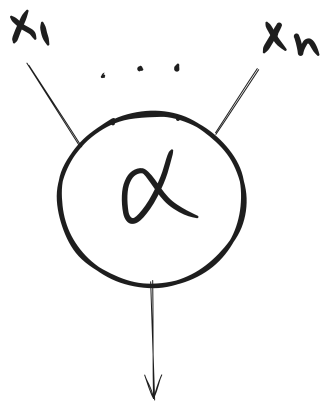
\includegraphics[width=0.3\linewidth]{figures/in_agent.pdf}
            \end{center}
        \end{column}
    \end{columns}
    \begin{itemize}
        \item Если $\alpha \in \Sigma$ и $\ar(\alpha) = n \in \N$, то у $\alpha$ имеется $n+1$ портов: $n$ \textit{дополнительных} и один выделенный~--- \textit{главный}.
    \end{itemize}

\end{frame}

\begin{frame}
    \frametitle{Формальное определение Interaction Nets II/II}

    \begin{itemize}
        \item \textit{Сеть}~--- неориентированный граф с символами из $\Sigma$ в его вершинах
        \item Ребра соединяют порты вершин, в каждый порт приходит не более одного ребра
        \item Порт не соединенный ни с одним ребром~--- \textit{свободный}, множество таких портов~--- \textit{интерфейс}
        \item Пара агентов $(\alpha, \beta) \in \Sigma \times \Sigma$, соединенных своими главными портами,~--- \textit{активная пара}
        \item Правило $((\alpha, \beta) \Longrightarrow N)$ заменяет активную пару $(\alpha, \beta)$ на сеть $N$.
        \item Для каждой пары агентов существует не более одного правила редукции, при этом в процессе редукции интерфейс сохраняется
    \end{itemize}

\end{frame}

\begin{frame}{Interaction Nets}

    \begin{center}
        \includegraphics[width=\textwidth]{figures/in_talk.pdf}
    \end{center}

\end{frame}

\begin{frame}
    \frametitle{Схема трансляции\footnote[frame]{По материалам Sinot F.-R. Call-by-Name and Call-by-Value as Token-Passing Interaction Nets // Typed Lambda Calculi and Applications Lecture Notes in Computer Science. / под ред. P. Urzyczyn. Berlin, Heidelberg: Springer Berlin Heidelberg, 2005. С. 386–400.}}

    Пусть $\mathcal{T}(\cdot)$~--- трансляция

    \begin{description}
        \item[Переменные] Переменные представляются проводами, поскольку рассматриваются только замкнутые термы

    \end{description}
    \begin{onlyenv}<1>
        \begin{columns}[totalwidth=\textwidth]
            \begin{column}{0.6\linewidth}
                \begin{description}
                    \item[Применение] Для применения $\mathcal{T}(t\ u)$ генерируется агент $a$, а к его портам подключаются результаты $\mathcal{T}(t)$ и $\mathcal{T}(u)$.
                          Если множество свободных переменных $t$ и $u$ не пусто, то для общих переменных генерируются агенты-дупликаторы $c$
                \end{description}
            \end{column}
            \begin{column}{0.4\linewidth}
                \begin{center}
                    \includegraphics[width=0.5\linewidth]{figures/sinot_app.pdf}
                \end{center}
            \end{column}
        \end{columns}
    \end{onlyenv}

    \begin{onlyenv}<2>
        \begin{columns}[totalwidth=\textwidth]
            \begin{column}{0.6\linewidth}
                \begin{description}
                    \item[Абстракция] Для абстракции $\mathcal{T}(\lambda x.t)$ генерируется агент $\lambda$, правый порт которого связывается с $\mathcal{T}(t)$, а левый с проводом, соответствующим $x$
                \end{description}
            \end{column}
            \begin{column}{0.4\linewidth}
                \begin{center}
                    \includegraphics[width=0.4\linewidth]{figures/sinot_abs_1.pdf}
                \end{center}
            \end{column}
        \end{columns}
    \end{onlyenv}

    \begin{onlyenv}<3>
        \begin{columns}[totalwidth=\textwidth]
            \begin{column}{0.6\linewidth}
                \begin{description}
                    \item[Абстракция] Для абстракции $\mathcal{T}(\lambda x.t)$ генерируется агент $\lambda$, правый порт которого связывается с $\mathcal{T}(t)$, если $x$ не содержится в $t$, то генерируется агент-уничтожитель $\varepsilon$
                \end{description}
            \end{column}
            \begin{column}{0.4\linewidth}
                \begin{center}
                    \includegraphics[width=0.5\linewidth]{figures/sinot_abs_2.pdf}
                \end{center}
            \end{column}
        \end{columns}
    \end{onlyenv}
\end{frame}

\end{document}
